\documentclass[conference]{IEEEtran}
\IEEEoverridecommandlockouts

% --- Packages (consistent with first file) ---
\usepackage{setspace}
\usepackage{gensymb}
\singlespacing
\usepackage[cmex10]{amsmath}
\usepackage{amsthm}
\usepackage{mathrsfs}
\usepackage{txfonts}
\usepackage{stfloats}
\usepackage{bm}
\usepackage{cite}
\usepackage{cases}
\usepackage{subfig}
\usepackage{longtable}
\usepackage{multirow}
\usepackage{enumitem}
\usepackage{mathtools}
\usepackage{tikz}
\usepackage{circuitikz}
\usepackage{verbatim}
\usepackage[breaklinks=true]{hyperref}
\usepackage{tkz-euclide}
\usepackage{listings}
\usepackage{color}
\usepackage{array}
\usepackage{calc}
\usepackage{hhline}
\usepackage{ifthen}
\usepackage{lscape}
\usepackage{chngcntr}
\usepackage{algorithm}
\usepackage[indLines=false]{algpseudocodex}

% --- Custom Math Commands (from first file) ---
\DeclareMathOperator*{\Res}{Res}
\renewcommand\thesection{\arabic{section}}
\renewcommand\thesubsection{\thesection.\arabic{subsection}}
\renewcommand\thesubsubsection{\thesubsection.\arabic{subsubsection}}
\renewcommand\thetable{\arabic{table}}
\hyphenation{op-tical net-works semi-conduc-tor}
\def\inputGnumericTable{}

\newtheorem{theorem}{Theorem}[section]
\newtheorem{problem}{Problem}
\newtheorem{proposition}{Proposition}[section]
\newtheorem{lemma}{Lemma}[section]
\newtheorem{corollary}[theorem]{Corollary}
\newtheorem{example}{Example}[section]
\newtheorem{definition}[problem]{Definition}
\theoremstyle{remark}
\newtheorem{rem}{Remark}

\newcommand{\BEQA}{\begin{eqnarray}}
	\newcommand{\EEQA}{\end{eqnarray}}
\providecommand{\mbf}{\mathbf}
\providecommand{\pr}[1]{\ensuremath{\Pr\left(#1\right)}}
\providecommand{\qfunc}[1]{\ensuremath{Q\left(#1\right)}}
\providecommand{\sbrak}[1]{\ensuremath{{}\left[#1\right]}}
\providecommand{\lsbrak}[1]{\ensuremath{{}\left[#1\right.}}
\providecommand{\rsbrak}[1]{\ensuremath{{}\left.#1\right]}}
\providecommand{\brak}[1]{\ensuremath{\left(#1\right)}}
\providecommand{\lbrak}[1]{\ensuremath{\left(#1\right.}}
\providecommand{\rbrak}[1]{\ensuremath{\left.#1\right)}}
\providecommand{\cbrak}[1]{\ensuremath{\left\{#1\right\}}}
\providecommand{\lcbrak}[1]{\ensuremath{\left\{#1\right.}}
\providecommand{\rcbrak}[1]{\ensuremath{\left.#1\right\}}}
\newcommand{\sgn}{\mathop{\mathrm{sgn}}}
\providecommand{\abs}[1]{\left\vert#1\right\vert}
\providecommand{\res}[1]{\Res\displaylimits_{#1}} 
\providecommand{\norm}[1]{\left\lVert#1\right\rVert}
\providecommand{\mtx}[1]{\mathbf{#1}}
\providecommand{\mean}[1]{E\left[ #1 \right]}   
\providecommand{\fourier}{\overset{\mathcal{F}}{ \rightleftharpoons}}
\providecommand{\system}[1]{\overset{\mathcal{#1}}{ \longleftrightarrow}}
\newcommand{\solution}{\noindent \textbf{Solution: }}
\newcommand{\cosec}{\,\text{cosec}\,}
\providecommand{\dec}[2]{\ensuremath{\overset{#1}{\underset{#2}{\gtrless}}}}
\newcommand{\myvec}[1]{\ensuremath{\begin{pmatrix}#1\end{pmatrix}}}
\newcommand{\mydet}[1]{\ensuremath{\begin{vmatrix}#1\end{vmatrix}}}
\renewcommand{\vec}[1]{\boldsymbol{\mathbf{#1}}}

% --- Document Begins ---
\begin{document}
	
	\title{A Logo for Narayanpal}
	\author{
		\IEEEauthorblockN{G.V.V. Sharma} 
			\IEEEauthorblockA{Department of Electrical Engineering, 
				\\
				Indian Institute of Technology Hyderabad,\\
				Kandi, India 502284
				\\
				gadepall@ee.iith.ac.in}
		}
	\maketitle
	
\begin{abstract}
	This paper determines the parameter pairs $(a, b)$ for the function $f(t) = e^{-at}u(t) + e^{bt}u(-t)$, subject to normalization, such that these pairs correspond to the endpoints of the latus recta of an associated conic. The work derives the conic equation binding the parameters, applies eigen-decomposition, and uses affine transformations to identify the valid $(a, b)$ values. Additionally, a numerical gradient descent method is proposed to determine symmetric truncation points $\theta = (\theta_0, \theta_1)$ such that the areas under $f(t)$ on either side of $t=0$ are equal. This approach allows for a flexible choice of the truncation window.
\end{abstract}



	\section{Question}
	Given that
	\begin{align}
		f(t) &= e^{-at}u(t) + e^{bt}u(-t) \label{q1}\\
		u(t) &= \begin{cases}
			0, & t<0\\
			\frac{1}{2}, & t=0 \\
			1, & t>0
		\end{cases} \label{q2}\\
		\int_{-\infty}^{\infty} f(t) &= 1 \label{q3}
	\end{align}
	
	Find the possible values of $(a,b)$ if these are the end points of the latus recta of the associated conic. Plot $f(t)$ for these values of $(a,b)$.
	
	\section{Solution}
	We expand the integral as 
	\begin{align}
		\int_{-\infty}^{\infty} f(t) &= \int_{-\infty}^{0} f(t) + \int_{0}^{\infty} f(t)\\
		&= \int_{-\infty}^{0} e^{bt} + \int_{0}^{\infty} e^{-at}\\
		&= \frac{1}{b} + \frac{1}{a} \label{integral_result}
	\end{align}
	Substituting \eqref{q3} in \eqref{integral_result}:
	\begin{align}
		\frac{1}{a} + \frac{1}{b} &= 1\\
		ab - a - b &= 0 \label{conic_ab}
	\end{align}
	This is the equation of a conic. If we take $a$ as $x$ and $b$ as $y$ and express this as a conic in standard form, we get
	\begin{align}
		\text{g}(\vec{x}) = \vec{x}^\text{T}\vec{Vx} + 2\vec{u}^\text{T}\vec{x} + f \label{actual_conic}
	\end{align}
	By comparison:
	\begin{align}
		\vec{V} &= \myvec{0 & \frac{1}{2} \\ \frac{1}{2} & 0}\\
		\vec{u} &= \myvec{-\frac{1}{2} \\ -\frac{1}{2}}\\
		f &= 0
	\end{align}
	We eigen-decompose $\vec{V}$ as 
	\begin{align}
		\vec{V} &= \vec{PDP}^\text{T}\\
		\vec{P} &= \myvec{\frac{1}{\sqrt{2}} & \frac{-1}{\sqrt{2}} \\ \frac{1}{\sqrt{2}} & \frac{1}{\sqrt{2}}}\\
		\vec{D} &= \myvec{\frac{1}{2} & 0 \\ 0 & \frac{-1}{2}}
	\end{align}
	Convert the conic into a standard conic using affine transformations.
	\begin{align}
		\vec{y}^\text{T}\brak{\frac{\vec{D}}{f_0}}\vec{y} &= 1\\
		\vec{x} &= \vec{Py} + \vec{c} \label{t1}
	\end{align}
	Where 
	\begin{align}
		f_0 &= \vec{u}^\text{T}\vec{V}^{-1}\vec{u} - f = 1\\
		\vec{c} &= -\vec{V}^{-1}\vec{u} = \myvec{1 \\ 1}
	\end{align}
	The eigenvalues of $\vec{D}$ are $\lambda_1 = \frac{1}{2}$, $\lambda_2=-\frac{1}{2}$. Using a reflection matrix and further transformation, we get the hyperbola in standard form:
	\begin{align}
		\vec{z}^\text{T}\brak{\frac{\vec{D_0}}{f_0}}\vec{z} &= 1\\
		j(\vec{z}) = \vec{z}^\text{T}\vec{D_0}\vec{z} - f_0 &= 0  \label{standard_conic}\\
		\vec{y} &= \vec{P}_0\vec{z} \label{t2}
	\end{align}
	Here $\vec{P}_0 = \myvec{0 & 1 \\ 1 & 0}$ and $\vec{D}_0 = \myvec{\frac{-1}{2} & 0 \\ 0 & \frac{1}{2}}$.
	
	Now, solve for the endpoints of the latus recta:
	\begin{align}
		\vec{n} &= \sqrt{\lambda_2}\vec{p}_1 = \myvec{0 \\ \frac{1}{\sqrt{2}}}\\
		e &= \sqrt{2}\\
		c &= \pm \frac{1}{\sqrt{2}}\\
		\vec{F} &= \pm 2 \vec{e}_2
	\end{align}
	Equation of latus recta:
	\begin{align}
		\vec{n}^\text{T}\vec{x} &= \vec{n}^\text{T}\vec{F}\\
		\equiv \vec{x} &= \vec{h} + k\vec{m} \label{latus_rectum}\\
		\vec{h} &= \myvec{0 \\ \pm 2}\\
		\vec{m} &= \myvec{1 \\ 0}
	\end{align}
	Let $\vec{\hat{z}}$ be the endpoints of the latus recta:
	\begin{align}
		k &= \pm \sqrt{2}\\
		\therefore \vec{\hat{z}} &= \myvec{\pm \sqrt{2} \\ \pm 2}
	\end{align}
	Transforming back to the original conic:
	\begin{align}
		\vec{\hat{x}} &= \vec{P}\brak{\vec{P}_0 \vec{\hat{z}}} + \vec{c}
	\end{align}
	Which gives:
	\begin{align*}
		\vec{\hat{x}}_1 &= \myvec{2+\sqrt{2} \\ \sqrt{2}}\\
		\vec{\hat{x}}_2 &= \myvec{\sqrt{2} \\ 2+\sqrt{2}}\\
		\vec{\hat{x}}_3 &= \myvec{2-\sqrt{2} \\ -\sqrt{2}}\\
		\vec{\hat{x}}_4 &= \myvec{-\sqrt{2} \\ 2-\sqrt{2}}
	\end{align*}
	Only $\vec{\hat{x}}_1$ and $\vec{\hat{x}}_2$ are valid as negative $a$ or $b$ will not yield a finite $f(t)$.
	
	\section{Plots}
	\begin{figure}[H]
		\centering
		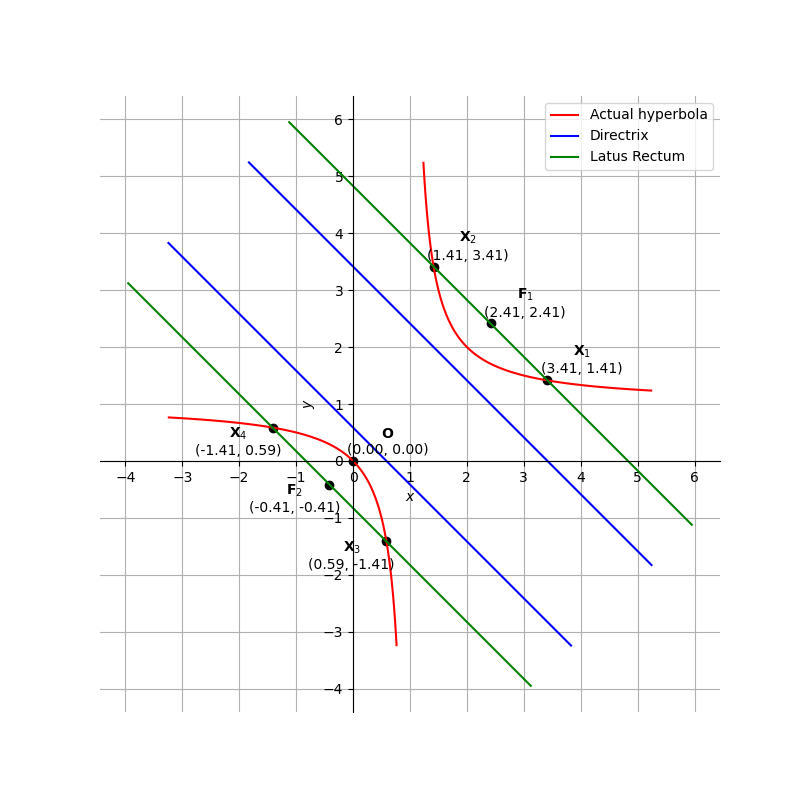
\includegraphics[width=1.2\columnwidth]{figs/Hyperbola.png} 
		\caption{Conic Section}
		\label{fig:Hyperbola}
	\end{figure}
	
	\begin{figure}[H]
		\centering
		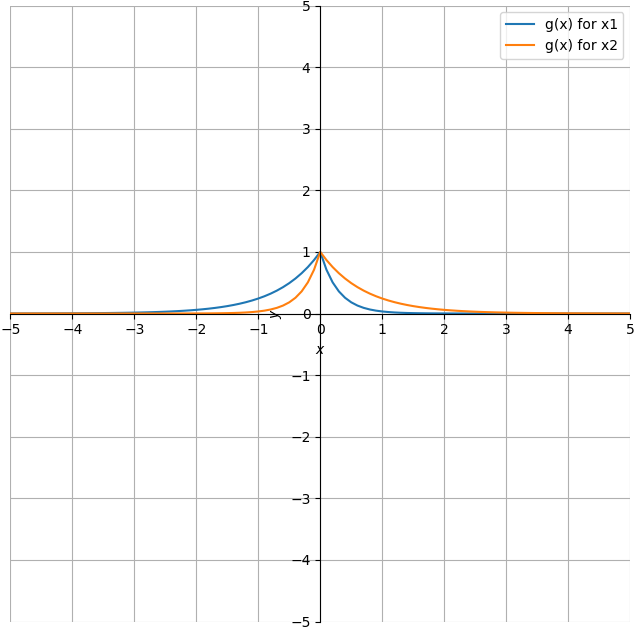
\includegraphics[width=1\columnwidth]{figs/function.png} 
		\caption{Function $f(t)$ for valid $(a, b)$}
		\label{fig:Function}
	\end{figure}
	
	\section{Numerical Area Balancing and Gradient Descent}
	We need to find the endpoints $(\theta_0, \theta_1)$ and truncate the function f(t), such that the the area under $f(t)$ is symmetric about $t=0$. For this, we will use gradient descent so that we get the closest solution to our guess.
	
	Define:
	\begin{align}
		A_L(\theta_0) &= \int_{\theta_0}^{0} e^{bt} \, dt = \frac{1 - e^{b\theta_0}}{b} \\
		A_R(\theta_1) &= \int_{0}^{\theta_1} e^{-at} \, dt = \frac{1 - e^{-a\theta_1}}{a}
	\end{align}
	
	We seek $\theta = (\theta_0, \theta_1)$ such that $A_L(\theta_0) = A_R(\theta_1)$. Rearranging:
	\begin{align}
		\frac{1 - e^{b\theta_0}}{b} - \frac{1 - e^{-a\theta_1}}{a} = 0
	\end{align}
	
	This nonlinear equation cannot be solved analytically in closed form. Thus, we define a cost function:
	\begin{align}
		\mathcal{C}(\theta) =\left(  \frac{1 - e^{b\theta_0}}{b} - \frac{1 - e^{-a\theta_1}}{a} \right) ^ 2
	\end{align}
	
	We minimize this cost using gradient descent:
	\begin{align}
		\frac{d\mathcal{C}}{d\theta_0} &= -\left(  \frac{1 - e^{b\theta_0}}{b} - \frac{1 - e^{-a\theta_1}}{a} \right) e^{b\theta_0} \\
		\frac{d\mathcal{C}}{d\theta_1} &= -\left(  \frac{1 - e^{b\theta_0}}{b} - \frac{1 - e^{-a\theta_1}}{a} \right) e^{-a\theta_1}
	\end{align}
	
	The update rule becomes:
	\begin{align}
		\theta_{n+1} \leftarrow \theta_{n} - \eta \cdot \nabla \mathcal{C}(\theta_n)
	\end{align}
	where $\eta$ is a learning rate.
	
	We initialize $\theta$ with a reasonable estimate and iterate until $|\mathcal{C}(\theta)| < 10^{-10}$. The resulting $\theta$ yields a numerically balanced integral under $f(t)$ on both sides of the origin.
	
	\begin{align}
		\theta_{(0)} = [-2, 3]^\text{T} \rightarrow \theta_{n} = [-0.37815999 , 3.00038288]^\text{T}
	\end{align}
	
	\begin{figure}[H]
		\centering
		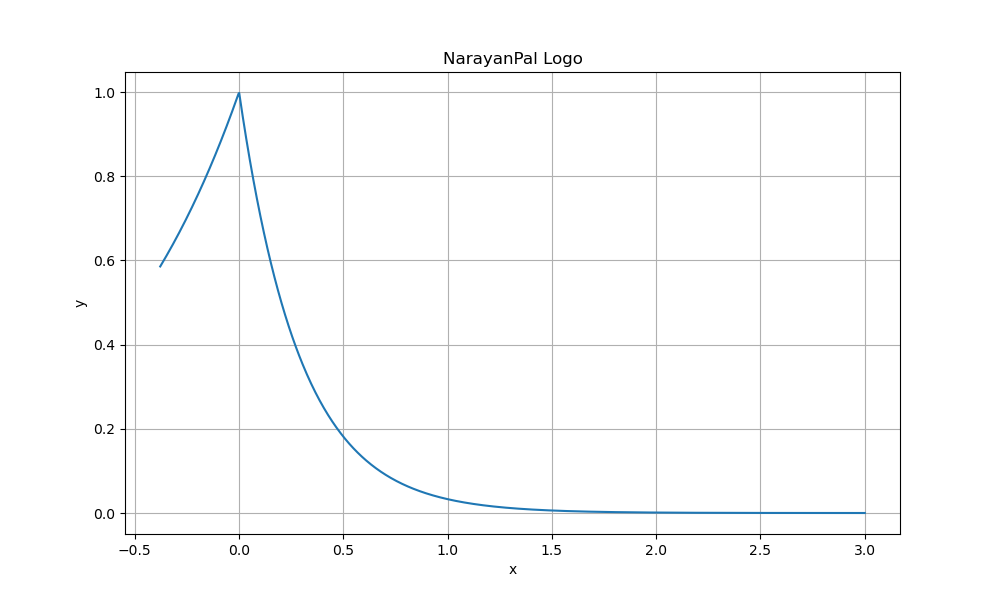
\includegraphics[width=1\columnwidth]{figs/window.png} 
		\caption{Truncated Function $f(t)$ }
		\label{fig:Window}
	\end{figure}
	
	
	
	
	% Bibliography style
	\bibliographystyle{IEEEtran}
	
\end{document}
